% Part 2 chapter carrying the observational side of "Dark Energy Evolution and the Far Future of an IAM Universe" (Feb 2026). Read in
% full 2026-10-02 (PDF text 590 lines in this extraction, 609 in the check file's; every line read). Chapter ch:darkenergy (p2_11) already carries
% the derivation of w_info, the two-ruler rates and the maturity table from the same paper; this chapter does not repeat them and carries the rest:
% w(z) through time, how much of it is observable, the CPL image and its sign, the three clocks, the no-Big-Rip bound and the tests.
% Numbers: docs/verification/scripts/verify_wz_far_future.py and verify_obs_chapters.py (section G). Check: observations/WZ_FAR_FUTURE_CHECK.md;
% errata WZ1-WZ7, V5. Heat-death arguments 2-3 are interpretation (Part 5).
\chapter{The equation of state through time, and the far future}\label{ch:wzfuture}

\section*{The place}
The cosmic horizon, at $T_{GH}=\hbar H/2\pi k_B$, holding the record $S_{\rm info}$ that matter writes as it collapses (Chapter~\ref{ch:surfaces}).
Chapter~\ref{ch:darkenergy} derived the equation of state of that record, $w_{\rm info}=-1-1/(3a)$, from $\rho_{\rm info}\propto E(a)$ and energy
conservation, and showed that it belongs to the matter-sector rate, not to the distances measured with light. This chapter follows it through time:
how phantom it is, how much of it any survey could see, and how it ends.

\section{$w$ through time}
With $a=1/(1+z)$, $w_{\rm info}(z)=-1-(1+z)/3$. The density it describes is $\rho_{\rm info}=\beta_mE(a)\rho_{\rm crit,0}$, so its weight against
$\rho_\Lambda$ falls as fast as $E(a)$ into the past. \calc
\begin{center}\small\begin{tabular}{lccc}\toprule
$z$ & $w_{\rm info}$ & $\rho_{\rm info}/\rho_\Lambda$ & $\rho_{\rm info}/(\rho_\Lambda+\rho_{\rm info})$\\\midrule
0 & $-1.333$ & 0.230 & 0.187\\ 0.5 & $-1.500$ & 0.140 & 0.122\\ 1 & $-1.667$ & 0.085 & 0.078\\ 2 & $-2.000$ & 0.031 & 0.030\\
3 & $-2.333$ & 0.011 & 0.011\\ $a\to\infty$ & $-1$ & 0.626 & 0.385\\\bottomrule
\end{tabular}\end{center}
The strongly phantom early values have almost nothing to act on: at $z=3$ the informational density is $1.1\,\%$ of $\rho_\Lambda$. A high-redshift
probe of $w$ cannot see them. Today the informational term is $18.7\,\%$ of the vacuum-like total and $23\,\%$ of $\rho_\Lambda$; at saturation,
$E\to e$, it reaches $0.626\,\rho_\Lambda$.
\begin{figure}[htbp]\centering
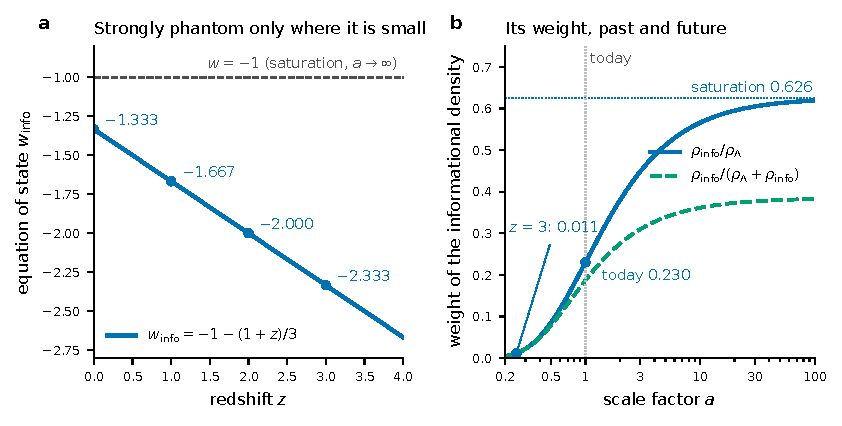
\includegraphics[width=\textwidth]{figures/part2/fig_wz_history.pdf}
\caption[The equation of state of the record and its weight through time]{(a) $w_{\rm info}(z)=-1-(1+z)/3$, which tends to $-1$ as $a\to\infty$. (b) The weight of the informational density, $\rho_{\rm info}/\rho_\Lambda=\beta_mE(a)/\Omega_\Lambda$ and its share of the vacuum-like total, from $a=0.2$ to $a=100$: 0.011 at $z=3$, 0.230 today, 0.626 at saturation. $H_0=67.4$, $\Omega_m=0.315$, $\beta_m=0.3153/2$. \calc}\label{fig:wz_history}
\end{figure}

\section{The CPL image and its sign}
Matching the value and first derivative of $w_{\rm info}$ at $a=1$ to $w(a)=w_0+w_a(1-a)$~\cite{ChevallierPolarski2001,Linder2003} gives
\begin{equation}w_0=-\tfrac43,\qquad w_a=-\left.\frac{dw_{\rm info}}{da}\right|_{a=1}=-\tfrac13 .\label{eq:wz_cpl}\end{equation}
\calc\ $w_a$ is negative. The equation of state rises with time, $dw/da=1/(3a^2)>0$, so it becomes less phantom as the universe expands. Against the DESI DR2
fits listed in Chapter~\ref{ch:darkenergy}~\cite{DESI2025}, Eq.~\eqref{eq:wz_cpl} is $9.0$, $7.6$ and $10.2\sigma$ away in $w_0$ (Pantheon+, Union3, DES Y5)
and $1.4$--$2.6\sigma$ in $w_a$. \calc\ As shown there, that distance is not a test: DESI's fits use distances measured with light, on which the informational term predicts $w=-1$; $w_{\rm info}$ belongs to the matter-sector rate. The
comparison that tests the term is the two-ruler one (Chapter~\ref{ch:sectortension}).

\section{Three clocks}
How fast the record is being written depends on the clock. Chapter~\ref{ch:darkenergy} gave two clocks: per e-fold of expansion, $dE/d\ln a=E/a$
peaks at $a=1$, the inflection of $E$ in $\ln a$; per unit cosmic time, $dE/dt=HE/a$ peaked at $z=1.26$, $8.9$~Gyr ago, at $3.38\,\%$ of the eventual
total per Gyr, and is $2.54\,\%$ per Gyr now. In the third clock, per unit scale factor, $d(E/e)/da=E/(e\,a^2)$ peaks at $a=0.5$ ($z=1$). \calc
``Today is the epoch of fastest writing'' therefore holds per e-fold only.
$E(1)=1$ because $1-1/a=0$ at $a=1$; it is today's normalisation, not a choice of reference epoch.
\begin{figure}[htbp]\centering
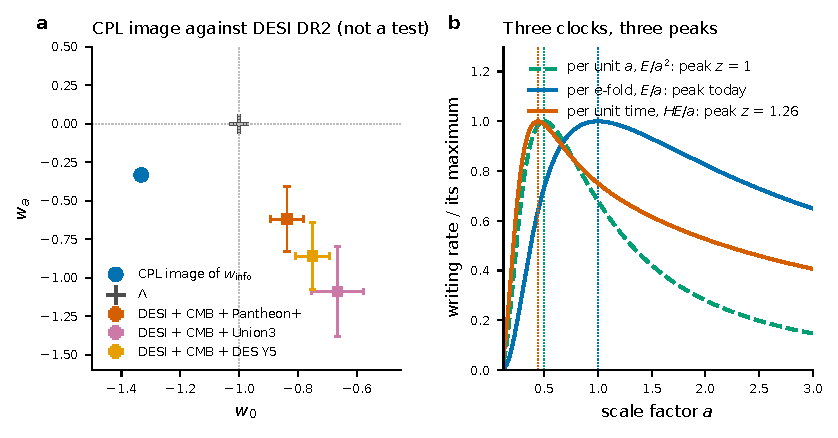
\includegraphics[width=\textwidth]{figures/part2/fig_wz_cpl_clocks.pdf}
\caption[The CPL image of the record term, and its writing rate in three clocks]{(a) The CPL image $(w_0,w_a)=(-\tfrac43,-\tfrac13)$ of $w_{\rm info}$ beside the DESI DR2 fits with the CMB and Pantheon+, Union3 or DES Y5 supernovae~\cite{DESI2025} (1$\sigma$ on each axis) \observed. The fits use light-ruler distances, on which the term predicts $w=-1$; the comparison is not a test. (b) The writing rate of $E(a)$ per unit $a$ (peak at $a=0.5$), per e-fold (peak today) and per unit cosmic time (peak at $z=1.26$), each normalised to its maximum. \calc}\label{fig:wz_cpl_clocks}
\end{figure}

\section{No Big Rip}
A Big Rip needs a phantom density that grows without bound, as for constant $w<-1$~\cite{Caldwell2002,Caldwell2003}. Here
\begin{equation}\frac{dw_{\rm info}}{da}=\frac{1}{3a^2}>0,\qquad\rho_{\rm info}(a)\le e\,\rho_{\rm info}(1),\label{eq:wz_norip}\end{equation}
so the density is bounded by $e$ times its present value and the equation of state tends to $-1$ from below. No phantom divergence occurs at any epoch.
\derived\ The bound follows from $E(a)\le e$ alone; no scalar field is introduced.

\section{The far future}
As in Chapter~\ref{ch:darkenergy}, the background is $\Lambda$CDM, so the photon-sector rate settles at $H_\infty=H_0\sqrt{\Omega_\Lambda}=55.78~\mathrm{km\,s^{-1}\,Mpc^{-1}}$ ($H_0=67.4$)
and the far future of the light sector is the de~Sitter state of $\Lambda$CDM. The matter-sector rate settles at $H_0\sqrt{\Omega_\Lambda+\beta_me}=71.12$.
\calc\ What ends is the writing: $E\to e$, structure formation stops, and the record on the horizon is complete; the informational term then behaves as a
constant, $w\to-1$. Whether that end state differs physically from the heat death of $\Lambda$CDM is a question of interpretation and is taken up in
Part~\ref{part:5}. \interp

\section{Tests}
\begin{itemize}
\item \emph{Two rulers.} The expansion history measured with matter (distance ladder, sirens, peculiar velocities) against the history measured with
light, redshift by redshift: $H_m/H=1.076$ today, rising to $1.275$ as $a\to\infty$ (Chapter~\ref{ch:darkenergy}). \prediction
\item \emph{One function twice.} The same $E(a)$ sets the growth weakening ($f\sigma_8$ low by $4.25\,\%$ today, Chapter~\ref{ch:surveys}) and the
matter-ruler expansion. A survey that measures both tests one curve twice. \prediction
\item \emph{Light-ruler distances follow $w=-1$.} Distances requiring $w\neq-1$, if confirmed, are not produced by this term. \prediction
\item \emph{Falsifier.} Matter-ruler data that require $w>-1$ where the term predicts $w_{\rm info}<-1$. No such comparison has been made yet. \openprob
\end{itemize}

\section{Status}
\begin{center}\small\begin{tabularx}{\linewidth}{>{\raggedright\arraybackslash}Xl}\toprule
Result & Label\\\midrule
$w_{\rm info}(z)=-1-(1+z)/3$; $\rho_{\rm info}/\rho_\Lambda$ through time & \calc\\
CPL image $(-\tfrac43,-\tfrac13)$; offsets from DESI DR2 (not a test) & \calc\\
Peak writing rate in three clocks & \calc\\
No Big Rip, $\rho_{\rm info}\le e\,\rho_{\rm info}(1)$ & \derived\\
Asymptotic rates $55.78$ (light) and $71.12$ (matter) & \calc\\
Two-ruler test; one $E(a)$ in growth and expansion & \prediction\\
Comparison with matter-ruler data & \openprob\\
End state versus heat death & \interp\\\bottomrule
\end{tabularx}\end{center}
